\iffalse

\documentclass[journal,10pt,twocolumn]{article}
\usepackage{graphicx}
\usepackage[margin=0.5in]{geometry}
\usepackage[cmex10]{amsmath}
\usepackage{array}
\usepackage{booktabs}
\usepackage{mathtools}
\usepackage{amssymb}
\title{\textbf{Conics Assignment}}
\author{lakshmi kamakshi}
\date{September 2022}
\providecommand{\norm}[1]{\left\lVert#1\right\rVert}
\providecommand{\abs}[1]{\left\vert#1\right\vert}
\let\vec\mathbf
\newcommand{\myvec}[1]{\ensuremath{\begin{pmatrix}#1\end{pmatrix}}}
\newcommand{\mydet}[1]{\ensuremath{\begin{vmatrix}#1\end{vmatrix}}}
\providecommand{\brak}[1]{\ensuremath{\left(#1\right)}}

\begin{document}

\maketitle
\paragraph{\textit{Problem Statement} -
\fi
An arch is in the form of a parabola with its axis vertical. The arch is 10m high and 5m wide at the base. How wide is it 2m from the vertex of the parabola?
\\
\solution
	\begin{figure}[!ht]
		\centering
 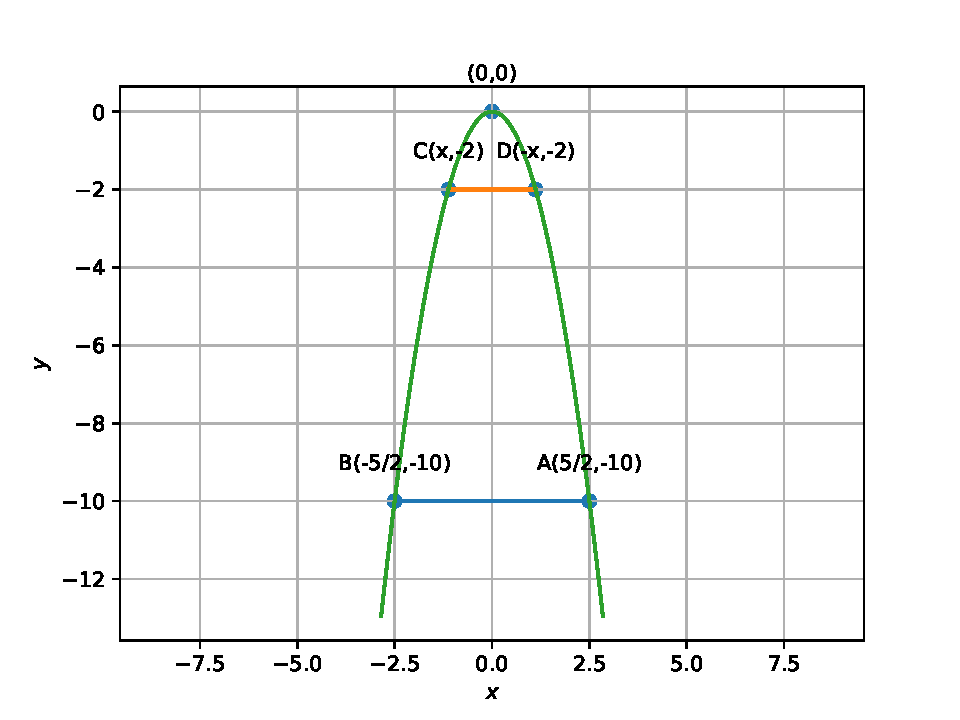
\includegraphics[width=\columnwidth]{chapters/11/11/5/2/figs/fig.pdf}
		\caption{}
		\label{fig:11/11/5/2}
  	\end{figure}
	\iffalse
} \vspace{5mm}

\section*{\large Solution}


Given, the axis of parabola is vertical,
\\ Let the equation of the axis be y-axis:
\begin{equation}
	\label{eq:parabola_q}
	\myvec{1\\0}\textbf{x}= 0
\end{equation}
\\ The above quadratic equation can be written in the general quadratic form as:

\begin{figure}[h]
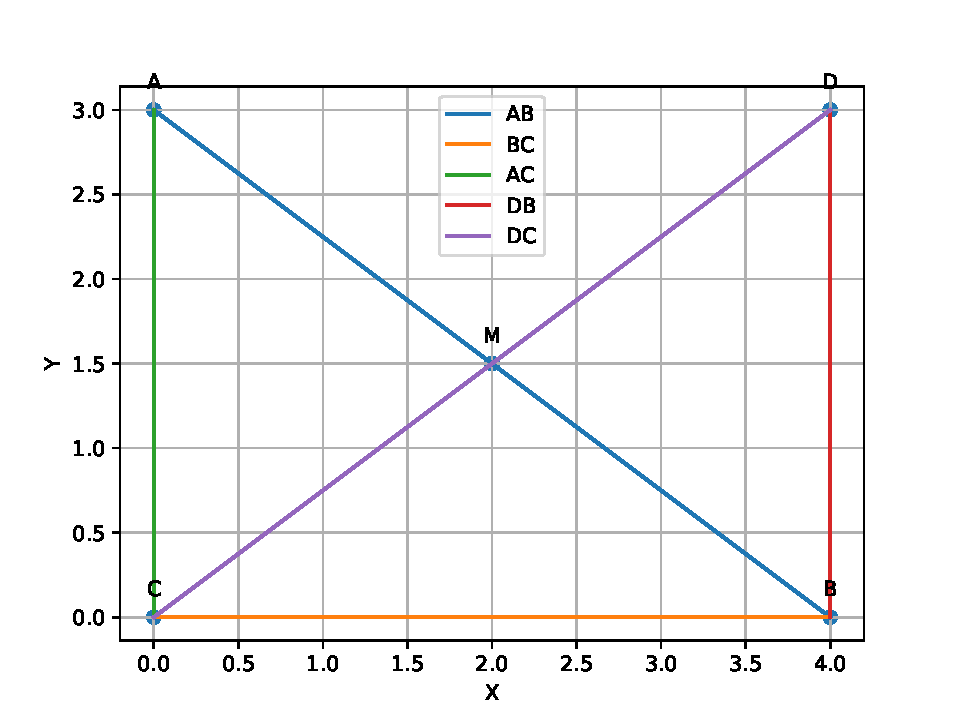
\includegraphics[width=0.8\columnwidth]{fig.pdf}
\end{figure}
\begin{equation}
	\label{eq:std_parabola}
	\textbf{x}^T\textbf{V}\textbf{x}+2\textbf{u}^T\textbf{x}+f=0
\end{equation}
where,
\begin{eqnarray}
\label{eq:Vec_V}
V = \myvec{1&0\\0&0}
\label{eq:Vec_U}
\\ u=\myvec{0\\2a}
\end{eqnarray}
\begin{equation}
\\ f =0
\end{equation}
Given arch is 10m high and 5m wide at the base. So the point $(\frac{5}{2},-10)$ lies on the parabola
\begin{equation}
	\myvec{X_1} = \myvec{\frac{5}{2}\\-10}
\end{equation}
\\ Substitute the point $X_1$ \\
\begin{eqnarray}
	\myvec{X_1}^T \myvec{V} \myvec{X_1} +2\myvec{u^T} \myvec{X_1} = 0
\\	a = \frac{5}{32}
\end{eqnarray}
\\Now , the matrix u will be,
\begin{equation}
	\myvec{u} = \myvec{0\\\frac{5}{16}}
\end{equation}
\\We need to find the width of parabola at a height of $2m$ from the vertex.So,the line parallel to x axis and passing through point $(0,-2)$ intersects the conic at 2 places C and D.
\\The line parallel to x-axis and passing through point $(0,-2)$ is
\begin{align}
	\myvec{X}\myvec{0\\1}^T = \myvec{2}
\end{align}
The points of intersection of the line 
\begin{align}
	L: \quad \vec{x} = \vec{q} + \mu \vec{m} \quad \mu \in \mathbf{R}
\label{eq:conic_tangent}
\end{align}
with the conic section  are given by
\begin{align}
\vec{x}_i = \vec{q} + \mu_i \vec{m}
\label{eq:conic_tangent_pts}
\end{align}
where 
{\tiny
\begin{multline}
\mu_i = \frac{1}
{
\vec{m}^T\vec{V}\vec{m}
}
\lbrak{-\vec{m}^T\brak{\vec{V}\vec{q}+\vec{u}}}
\\
\pm
\rbrak{\sqrt{
\sbrak{
\vec{m}^T\brak{\vec{V}\vec{q}+\vec{u}}
}^2
-
\brak
{
\vec{q}^T\vec{V}\vec{q} + 2\vec{u}^T\vec{q} +f
}
\brak{\vec{m}^T\vec{V}\vec{m}}
	}}
\label{eq:tangent_roots}
\end{multline}
}
\\
Substituting the line in the conic
\begin{align}
\brak{\vec{q} + \mu \vec{m}}^T\vec{V}\brak{\vec{q} + \mu \vec{m}}  
\\
+ 2 \vec{u}^T\brak{\vec{q} + \mu \vec{m}}+f &= 0
\\
\implies \mu^2\vec{m}^T\vec{V}\vec{m} + 2 \mu\vec{m}^T\brak{\vec{V}\vec{q}+\vec{u}} 
\\
+ \vec{q}^T\vec{V}\vec{q} + 2\vec{u}^T\vec{q} +f &= 0
\label{eq:conic_intercept}
\end{align}
Solving the above quadratic equations yeilds the roots.Let the point of intersections of line and curve be C and D.
\begin{align}
	C = q+ \mu_1m
	\\ D = q+ \mu_2m
\end{align}
\\The line CD will be
\begin{align}
	C-D = m(\mu_1-\mu_2)
	 \\ \textbf{m} = \myvec{1\\0}
\end{align}
The required width of parabola is the norm of the line CD.
\begin{align}
	||\boldsymbol{C-D}|| =
	2\sqrt{
\sbrak{
\vec{m}^T\brak{\vec{V}\vec{q}+\vec{u}}
}^2
-
\brak
{
\vec{q}^T\vec{V}\vec{q} + 2\vec{u}^T\vec{q} +f
}}
\end{align}
substitute the values of \vec{m},\vec{q},\vec{V} and \vec{u}
\begin{align}
	\frac{1}{2}||\vec{C-D}||^2 =
	\myvec{1&0}\brak{\vec{V}\myvec{0\\-2}+\vec{u}}\brak{\vec{V}\myvec{0\\-2}+\vec{u}}^T-
\end{align}
\begin{align*}
\brak
{
	\myvec{0&-2}\vec{V}\myvec{0\\-2} + 2\vec{u}^T\myvec{0\\-2} 
}
\end{align*}
 \begin{multiline}
	 \implies \sbrak{\myvec{1&0}\brak{\myvec{1&0\\0&0}\myvec{0\\-2} + \myvec{0\\\frac{5}{16}}}} \brak{\myvec{1&0\\0&0}\myvec{0\\-2} + \myvec{0\\\frac{5}{16}}}}^T  - \\
	 \\ \brak{\myvec{0&-2}\myvec{1&0\\0&0}\myvec{0\\-2} + 2\myvec{0 & \frac{5}{16}}\myvec{0\\-2} - 0} \\ \brak{\myvec{1&0}\myvec{1&0\\0&0}\myvec{1\\0}}
\end{multline}
\begin{align}
	\implies \sbrak{\myvec{1&0}\myvec{0\\\frac{5}{16}}}^2 - \brak{\myvec{0\\0}+2\myvec{0\\\frac{5}{-8}} - 0}(1) \\
 & = \myvec{5\\2}
\end{align}
\\The width of the Parabola at $2m$ height is the length of the line CD.  \begin{align} ||\vec{C-D}|| = \myvec{\sqrt{5}}$m$ \end{align} \section*{\large Construction} The input parameters are V,u,$X_1$,$y_2$ \\
\setlength\extrarowheight{7pt}
\begin{tabular}{|c|c|c|}
	\hline
	\textbf{Symbol}&\textbf{Value}&\textbf{Description}\\
	\hline
	$X_1$=\myvec{x_1\\y_1} & \myvec{\frac{5}{2}\\-10}&point at base \\[8pt]
	\hline
	$y_2$ & -2& height of point C\\[8pt]
	\hline
	$\vec{P}$&\myvec{0&1\\1&0}&eigenvectors of $\vec{V}$\\[8pt]
	\hline
	$\vec{c}$&$\myvec{0\\0}$&center of parabola\\
	\hline
	$\eta$&$\vec{u}^{\top}\vec{p}_1$&from Eq11\\[8pt]
	\hline
	$\lambda_2$&$\vec{e}_2^{\top}D\vec{e}_2$&from Eq9 \\[8pt]
	\hline
	$(\vec{A},\vec{B})$&\myvec{x_1&-x_1\\y_1&y_1}&points at the base\\[8pt]
	\hline
	$(\vec{C},\vec{D})$&\myvec{\sqrt{\frac{5y_2}{8}}&\sqrt{\frac{-5y_2}{8}}\\2&2}&points at 2m height\\[8pt]	\hline
\end{tabular}
\end{document}
\fi
